\documentclass{vkr}
\usepackage[english, russian]{babel} % переносы
\usepackage{graphicx} % для вставки картинок
\graphicspath{{images/}} % путь к изображениям
\usepackage[hidelinks]{hyperref}
\usepackage{float} % определяет метод H для рисунка с переносом на следующую страницу, ели не помещается
\usepackage{pdflscape}
\addto{\captionsrussian}{\renewcommand{\refname}{СПИСОК ИСПОЛЬЗОВАННЫХ ИСТОЧНИКОВ}}
\usepackage{xltabular} % для вставки таблиц
\usepackage{makecell}
\renewcommand\theadfont{} % шрифт в /thead
\usepackage{array} % для определения новых типов столбцов таблиц
\newcolumntype{T}{>{\centering\arraybackslash}X} % новый тип столбца T - автоматическая ширина столбца с выравниванием по центру
\newcolumntype{R}{>{\raggedleft\arraybackslash}X} % новый тип столбца R - автоматическая ширина столбца с выравниванием по правому краю
\newcolumntype{C}[1]{>{\centering\let\newline\\\arraybackslash\hspace{0pt}}m{#1}} % новый тип столбца C - фиксированная ширина столбца с выравниванием по центру
\newcolumntype{r}[1]{>{\raggedleft\arraybackslash}p{#1}} % новый тип столбца r - фиксированная ширина столбца с выравниванием по правому краю
\newcommand{\centrow}{\centering\arraybackslash} % командой \centrow можно центрировать одну ячейку (заголовок) в столбце типа X или p, оставив в оcтальных ячейках другой тип выравнивания
\newcommand{\finishhead}{\endhead\hline\endlastfoot}
\newcommand{\continuecaption}[1]{\caption*{#1}\\ \hline }
\usepackage{etoolbox}
\AtBeginEnvironment{xltabular}{\refstepcounter{tablecnt}} % подсчет таблиц xltabular, обычные таблицы подсчитываются в классе

\usepackage[tableposition=top]{caption} % подпись таблицы вверху
\captionsetup{strut=off}
\setlength{\intextsep}{0pt} % Vertical space above & below [h] floats
\setlength{\textfloatsep}{0pt} % Vertical space below (above) [t] ([b]) floats
\DeclareCaptionLabelFormat{gostfigure}{Рисунок #2} %подпись рисунка
\DeclareCaptionLabelFormat{gosttable}{Таблица #2} %подпись таблицы
\DeclareCaptionLabelSeparator{gost}{~--~} %разделитель в рисунках и таблицах
\captionsetup{labelsep=gost}
\captionsetup[figure]{aboveskip=10pt,belowskip=4mm,justification=centering,labelformat=gostfigure} % настройка подписи рисунка
\captionsetup[table]{font={stretch=1.41},skip=0pt,belowskip=0pt,aboveskip=8.5pt,singlelinecheck=off,labelformat=gosttable} % настройка подписи таблицы

\setlength{\LTpre}{8mm} % отступ сверху таблицы
\setlength{\LTpost}{6mm} % отступ снизу таблицы

\usepackage{enumitem}
\setlist{nolistsep,wide=\parindent,itemindent=*} % отступы вокруг списков, выравнивание с учетом разделителя

\usepackage{color} %% это для отображения цвета в коде
\usepackage{listings} %% листинги кода
\setmonofont[Scale=0.7]{Verdana} % моноширный шрифт для листинга

\definecolor{codegreen}{rgb}{0,0.6,0}
\definecolor{codegray}{rgb}{0.5,0.5,0.5}
\definecolor{codepurple}{rgb}{0.58,0,0.82}

\lstset{ %
language=C,                 % выбор языка для подсветки (здесь это С)
numbers=left,               % где поставить нумерацию строк (слева\справа)
numberstyle=\tiny,           % размер шрифта для номеров строк
stepnumber=1,                   % размер шага между двумя номерами строк
numbersep=5pt,                % как далеко отстоят номера строк от подсвечиваемого кода
commentstyle=\color{codegreen},
keywordstyle=\color{magenta},
numberstyle=\tiny\color{codegray},
stringstyle=\color{codepurple},
basicstyle=\linespread{0.95}\ttfamily,
backgroundcolor=\color{white}, % цвет фона подсветки - используем \usepackage{color}
showspaces=false,            % показывать или нет пробелы специальными отступами
showstringspaces=false,      % показывать или нет пробелы в строках
showtabs=false,             % показывать или нет табуляцию в строках
frame=single,              % рисовать рамку вокруг кода
tabsize=2,                 % размер табуляции по умолчанию равен 2 пробелам
captionpos=t,              % позиция заголовка вверху [t] или внизу [b] 
breaklines=true,           % автоматически переносить строки (да\нет)
breakatwhitespace=false, % переносить строки только если есть пробел
escapeinside={\%*}{*)}   % если нужно добавить комментарии в коде
}

\makeatletter % чтобы допускались русские комментарии в листингах
\lst@InputCatcodes
\def\lst@DefEC{%
 \lst@CCECUse \lst@ProcessLetter
  ^^80^^81^^82^^83^^84^^85^^86^^87^^88^^89^^8a^^8b^^8c^^8d^^8e^^8f%
  ^^90^^91^^92^^93^^94^^95^^96^^97^^98^^99^^9a^^9b^^9c^^9d^^9e^^9f%
  ^^a0^^a1^^a2^^a3^^a4^^a5^^a6^^a7^^a8^^a9^^aa^^ab^^ac^^ad^^ae^^af%
  ^^b0^^b1^^b2^^b3^^b4^^b5^^b6^^b7^^b8^^b9^^ba^^bb^^bc^^bd^^be^^bf%
  ^^c0^^c1^^c2^^c3^^c4^^c5^^c6^^c7^^c8^^c9^^ca^^cb^^cc^^cd^^ce^^cf%
  ^^d0^^d1^^d2^^d3^^d4^^d5^^d6^^d7^^d8^^d9^^da^^db^^dc^^dd^^de^^df%
  ^^e0^^e1^^e2^^e3^^e4^^e5^^e6^^e7^^e8^^e9^^ea^^eb^^ec^^ed^^ee^^ef%
  ^^f0^^f1^^f2^^f3^^f4^^f5^^f6^^f7^^f8^^f9^^fa^^fb^^fc^^fd^^fe^^ff%
  ^^^^20ac^^^^0153^^^^0152%
  % Basic Cyrillic alphabet coverage
  ^^^^0410^^^^0411^^^^0412^^^^0413^^^^0414^^^^0415^^^^0416^^^^0417%
  ^^^^0418^^^^0419^^^^041a^^^^041b^^^^041c^^^^041d^^^^041e^^^^041f%
  ^^^^0420^^^^0421^^^^0422^^^^0423^^^^0424^^^^0425^^^^0426^^^^0427%
  ^^^^0428^^^^0429^^^^042a^^^^042b^^^^042c^^^^042d^^^^042e^^^^042f%
  ^^^^0430^^^^0431^^^^0432^^^^0433^^^^0434^^^^0435^^^^0436^^^^0437%
  ^^^^0438^^^^0439^^^^043a^^^^043b^^^^043c^^^^043d^^^^043e^^^^043f%
  ^^^^0440^^^^0441^^^^0442^^^^0443^^^^0444^^^^0445^^^^0446^^^^0447%
  ^^^^0448^^^^0449^^^^044a^^^^044b^^^^044c^^^^044d^^^^044e^^^^044f%
  ^^^^0401^^^^0451%
  %%%
  ^^00}
\lst@RestoreCatcodes
\makeatother


% Режим шаблона (должен быть включен один из трех)
%\ВКРtrue
%\Практикаtrue
\Курсоваяtrue

\newcommand{\Дисциплина}{<<Проектирование и архитектура программных систем>>} % для курсовой
\newcommand{\КодСпециальности}{09.03.04} % Курсовая
\newcommand{\Специальность}{Программная инженерия} % Курсовая
\newcommand{\Тема}{Растровый графический редактор} % ВКР Курсовая
\newcommand{\ТемаВтораяСтрока}{ }
\newcommand{\ГдеПроводитсяПрактика}{Юго-Западном государственном университете} % для практики
\newcommand{\РуководительПрактПредпр}{Куркина А. В.} % для практики
\newcommand{\ДолжнРуководительПрактПредпр}{директор} % для практики
\newcommand{\РуководительПрактУнивер}{Чаплыгин А. А.} % для практики
\newcommand{\ДолжнРуководительПрактУнивер}{к.т.н. доцент} % для практики
\newcommand{\Автор}{И. В. Подушкин}
\newcommand{\АвторРод}{Подушкина И.В.}
\newcommand{\АвторПолностьюРод}{Иванова Ивана Ивановича} % для практики
\newcommand{\Шифр}{21-06-0135}
\newcommand{\Курс}{4} % для практики
\newcommand{\Группа}{ПО-11б}
\newcommand{\Руководитель}{А. А. Чаплыгин} % для ВКР и курсовой
\newcommand{\Нормоконтроль}{А. А. Чаплыгин} % для ВКР
\newcommand{\ЗавКаф}{А. В. Малышев} % для ВКР
\newcommand{\ДатаПриказа}{«07» апреля 2023~г.} % для ВКР
\newcommand{\НомерПриказа}{1505-с} % для ВКР
\newcommand{\СрокПредоставления}{«11» января 2024~г.} % для ВКР, курсового

\begin{document}
\maketitle
\ifПрактика{}\else{
   \newpage
\begin{center}
\large\textbf{Минобрнауки России}

\large\textbf{Юго-Западный государственный университет}
\vskip 1em
\normalsize{Кафедра программной инженерии}
\vskip 1em
\ifВКР{
        \begin{flushright}
        \begin{tabular}{p{.4\textwidth}}
        \centrow УТВЕРЖДАЮ: \\
        \centrow Заведующий кафедрой \\
        \hrulefill \\
        \setarstrut{\footnotesize}
        \centrow\footnotesize{(подпись, инициалы, фамилия)}\\
        \restorearstrut
        «\underline{\hspace{1cm}}»
        \underline{\hspace{3cm}}
        20\underline{\hspace{1cm}} г.\\
        \end{tabular}
        \end{flushright}
        }\fi
\end{center}
\vspace{1em}
  \begin{center}
  \large
\ifВКР{
ЗАДАНИЕ НА ВЫПУСКНУЮ КВАЛИФИКАЦИОННУЮ РАБОТУ
  ПО ПРОГРАММЕ БАКАЛАВРИАТА}
  \else
ЗАДАНИЕ НА КУРСОВУЮ РАБОТУ (ПРОЕКТ)
\fi
\normalsize
  \end{center}
\vspace{1em}
{\parindent0pt
  Студента \АвторРод, шифр\ \Шифр, группа \Группа
  
1. Тема «\Тема\ \ТемаВтораяСтрока»
\ifВКР{
утверждена приказом ректора ЮЗГУ от \ДатаПриказа\ № \НомерПриказа
}\fi.

2. Срок предоставления работы к защите \СрокПредоставления

3. Исходные данные для создания программной системы:

3.1. Перечень решаемых задач:}

\renewcommand\labelenumi{\theenumi)}

\begin{enumerate}
\item проанализировать другие графические редакторы;
\item разработать концептуальную модель графического редактора;
\item спроектировать программную систему графического редактора;
\item сконструировать и протестировать программную систему графического редактора.
\end{enumerate}

{\parindent0pt
  3.2. Входные данные и требуемые результаты для программы:}

\begin{enumerate}
\item Входными данными для программной системы являются: ввод пользователя.
\item Выходными данными для программной системы являются: изображение на экране.
\end{enumerate}

{\parindent0pt

  4. Содержание работы (по разделам):
  
  4.1. Введение
  
  4.1. Анализ предметной области
  
4.2. Техническое задание: основание для разработки, назначение разработки,
требования к программной системе, требования к оформлению документации.

4.3. Технический проект: общие сведения о программной системе, проект
данных программной системы, проектирование архитектуры программной системы, проектирование пользовательского интерфейса программной системы.

4.4. Рабочий проект: спецификация компонентов и классов программной системы, тестирование программной системы, сборка компонентов программной системы.

4.5. Заключение

4.6. Список использованных источников

5. Перечень графического материала:

\списокПлакатов

\vskip 2em
\begin{tabular}{p{6.8cm}C{3.8cm}C{4.8cm}}
Руководитель \ifВКР{ВКР}\else работы (проекта) \fi & \lhrulefill{\fill} & \fillcenter\Руководитель\\
\setarstrut{\footnotesize}
& \footnotesize{(подпись, дата)} & \footnotesize{(инициалы, фамилия)}\\
\restorearstrut
Задание принял к исполнению & \lhrulefill{\fill} & \fillcenter\Автор\\
\setarstrut{\footnotesize}
& \footnotesize{(подпись, дата)} & \footnotesize{(инициалы, фамилия)}\\
\restorearstrut
\end{tabular}
}

\renewcommand\labelenumi{\theenumi.}

   \abstract{РЕФЕРАТ}

Объем работы равен \formbytotal{lastpage}{страниц}{е}{ам}{ам}. Работа содержит \formbytotal{figurecnt}{иллюстраци}{ю}{и}{й}, \formbytotal{tablecnt}{таблиц}{у}{ы}{}, \arabic{bibcount} библиографических источников. Количество приложений – 1. Фрагменты исходного кода представлены в приложении А.

Перечень ключевых слов: графический редактор, интерфейс пользователя, инструменты рисования, обработка изображений, форматы файлов, растровая графика, классы, компонент, модуль, сущность, метод, пользователь.

Объектом разработки является графический редактор, включая его основные компоненты, функциональность, пользовательский интерфейс, инструменты рисования и редактирования, а также возможности обработки изображений.

Целью курсовой работы является разработка легкого в использовании графического редактора, ориентированный на широкий круг пользователей, предоставляющий базовый, но эффективный набор инструментов для создания и редактирования изображений.

В процессе создания сайта были выделены основные сущности путем создания информационных блоков, использованы классы и методы модулей, обеспечивающие работу с сущностями предметной области, а также корректную работу приложения, разработаны инструменты для взаимодействия с рабочей зоной программы.

При разработке сайта использовался язык программирования Python.

\selectlanguage{english}
\abstract{ABSTRACT}
  
The volume of work is \formbytotal{lastpage}{page}{}{s}{s}. The work contains \formbytotal{figurecnt}{illustration}{}{s}{s}, \formbytotal{tablecnt}{table}{}{s}{s}, \arabic{bibcount} bibliographic sources. The number of applications is 1. Fragments of the source code are presented in annex A.

The list of keywords: graphic editor, user interface, drawing tools, image processing, file formats, raster graphics, classes, component, module, entity, method, user.

The object of development is a graphic editor, including its main components, functionality, user interface, drawing and editing tools, as well as image processing capabilities.

The purpose of the course work is to develop an easy-to-use graphical editor aimed at a wide range of users, providing a basic but effective set of tools for creating and editing images.

In the process of creating the site, the main entities were identified by creating information blocks, classes and methods of modules were used to ensure work with the entities of the subject area, as well as the correct operation of the application, tools for interacting with the work area of the program were developed.

The Python programming language was used in the development of the site.
\selectlanguage{russian}
}\fi
\tableofcontents
\section*{ОБОЗНАЧЕНИЯ И СОКРАЩЕНИЯ}

ИТ -- информационные технологии. 

ПО -- программное обеспечение.

ГР -- графический редактор.

РГ -- растровая графика.

РП -- рабочий проект.

ТЗ -- техническое задание.

ТП -- технический проект.

UML (Unified Modelling Language) -- язык графического описания для объектного моделирования в области разработки программного обеспечения.

\ifПрактика{}\else{\section*{ВВЕДЕНИЕ}
\addcontentsline{toc}{section}{ВВЕДЕНИЕ}

Графические редакторы представляют собой мощные инструменты для создания, редактирования и обработки изображений, играя важную роль в современном мире визуального искусства и дизайна. Они предоставляют пользователю уникальные возможности воплощения творческих идей, преобразуя пиксели на экране в произведения искусства.

Эти программы обладают разнообразным функционалом, включая рисование, обрезку, ретушь, добавление эффектов, редактирование цветов и многое другое. В современных условиях графические редакторы предоставляют широкий спектр инструментов для создания и редактирования фотографий, иллюстраций, дизайна интерфейсов, баннеров и других графических элементов.

Adobe Photoshop, GIMP, CorelDRAW, и множество других программ являются стандартами в этой области, предоставляя профессионалам и любителям возможность воплощать свои творческие идеи. С развитием технологий, графические редакторы становятся все более доступными и интуитивно понятными, что позволяет широкому кругу пользователей экспериментировать с изобразительными возможностями.

Благодаря графическим редакторам творчество становится более доступным, а визуальное восприятие обогащается уникальными изображениями, которые олицетворяют индивидуальность и талант их создателей.

\emph{Цель настоящей работы} – создание собственного графического редактора, способного удовлетворить потребности пользователей в редактировании и обработке изображений. Для достижения поставленной цели необходимо решить \emph{следующие задачи:}
\begin{itemize}
\item провести анализ предметной области;
\item разработать концептуальную модель приложения;
\item спроектировать приложение;
\item реализовать приложение средствами языка программирования Python.
\end{itemize}

\emph{Структура и объем работы.} Отчет состоит из введения, 4 разделов основной части, заключения, списка использованных источников, 2 приложений. Текст выпускной квалификационной работы равен \formbytotal{page}{страниц}{е}{ам}{ам}.

\emph{Во введении} сформулирована цель работы, поставлены задачи разработки, описана структура работы, приведено краткое содержание каждого из разделов.

\emph{В первом разделе} на стадии описания технической характеристики приводятся сведения о предметной области выбранной темы, историю развития программного обеспечения в данной теме.

\emph{Во втором разделе} на стадии технического задания приводятся требования к разрабатываемому приложению.

\emph{В третьем разделе} на стадии технического проектирования представлены проектные решения для приложения.

\emph{В четвертом разделе} приводится список классов и их методов, использованных при разработке сайта, производится тестирование разработанного приложения.

В заключении излагаются основные результаты работы, полученные в ходе разработки.

В приложении А представлены фрагменты исходного кода. 
}\fi
\section{Анализ предметной области}
\subsection{Описание предметной области}

История графических редакторов берет свое начало во второй половине 20 века и прошла через ряд значимых этапов. Одним из ключевых моментов стало появление первых графических редакторов, среди которых выделяется Sketchpad, созданный в 1963 году Иваном Сазерлендом в MIT. Эта программа открыла новые горизонты в возможностях создания и редактирования изображений с использованием графического интерфейса.

В последующие десятилетия появились инновационные графические редакторы, в числе которых Adobe Photoshop, ставший отраслевым стандартом для обработки изображений. Программы также стали более доступными, что способствовало распространению графического дизайна и творчества.

С развитием технологий возникли новые возможности, такие как векторная графика и трехмерное моделирование. Инструменты, вроде Adobe Illustrator и Blender, предоставляют пользователям широкий спектр функций для творческой работы и дизайна.

Сегодня графические редакторы стали неотъемлемой частью повседневной жизни, используемой для создания и редактирования изображений, дизайна интерфейсов, анимации и других творческих задач. Их эволюция свидетельствует о постоянном стремлении к улучшению возможностей обработки графики и созданию интуитивных инструментов для пользователей.

В результате графические редакторы охватывают разнообразные области, включая дизайн, искусство, рекламу и веб-разработку. Их роль в современном мире выходит за пределы профессиональных студий, охватывая любителей и тех, кто желает воплотить свои творческие идеи в цифровой форме.
\subsection{Графические редакторы, их классификация}

\textbf{Растровый графический редактор} -- специализированная программа, предназначенная для создания и обработки растровых изображений, то есть графики, которая в память компьютера записывается как набор точек (пикселей), которые образуют строки и столбцы, например, точка задается своими координатами (Х, У).

Любой пиксель имеет фиксированное положение и цвет. Хранение каждого пикселя требует некоторого количества бит информации, которое зависит от количества цветов в изображении. Таким образом, качество растровых изображений зависит от их размера (числа пикселей по горизонтали и вертикали) и количества цветов, которые могут принимать пиксели.

Растровые графические редакторы позволяют пользователю рисовать и редактировать изображения на экране компьютера, а также сохранять их в различных растровых форматах, и больше подходят для обработки и ретуширования фотографий, создания фотореалистичных иллюстраций, коллажей, и создания рисунков от руки с помощью графического планшета.

\textbf{Векторный графический редактор} - это программа, предназначенная для создания изображений высокой точности, например, чертежи или схемы, создания разметки страниц, типографии, логотипов, мультипликация, сложные геометрические шаблоны, технических иллюстраций, создания диаграмм и составления блок-схем.

Главными основными инструментами в векторном редакторе являются кривые Безье, позволяющие рисовать кривые (ломаные, прямые и гладкие) по сегментам с точным размещением узловых (опорных) точек и контролем над формой каждого сегмента.


\section{Техническое задание}
\subsection{Основание для разработки}

Основанием для разработки программного продукта служит задание курсовой работы «Растровый графический редактор» по дисциплине «Языки объектно-ориентированного программирования».

\subsection{Цель и назначение разработки}

Основной задачей курсовой работы является разработка программного продукта для создания и редактирования графических изображений.

Задачами данной разработки являются:
\begin{itemize}
\item разработка архитектуры приложения;
\item реализация возможности создавать файл с графическим изображением;
\item разработка интерфейса приложения;
\item реализация возможности открывать, редактировать и сохранять файл с графическим изображением;
\item реализация возможности менять размер, создаваемого полотна;
\item реализация возможности наблюдать изменения, происходящие на экране, которые вызваны действиями пользователя;
\item реализация возможности изменять параметры кисти: размер, цвет;
\end{itemize}

\subsection{Требования пользователя к интерфейсу приложения}

Приложение должен включать в себя:
\begin{itemize}
	\item начальное окно с параметрами создаваемого холста;
	\item панель для работы с файлом: сохранение, удаление, открытие другого файла;
	\item панель для работы с инструментами: кисть, ластик.
	\item панель для работы с параметрами инструмента: цветом и размером;
\end{itemize}

Композиция шаблона приложения представлена на рисунке ~\ref{shablon:image}.

\begin{figure}[ht]
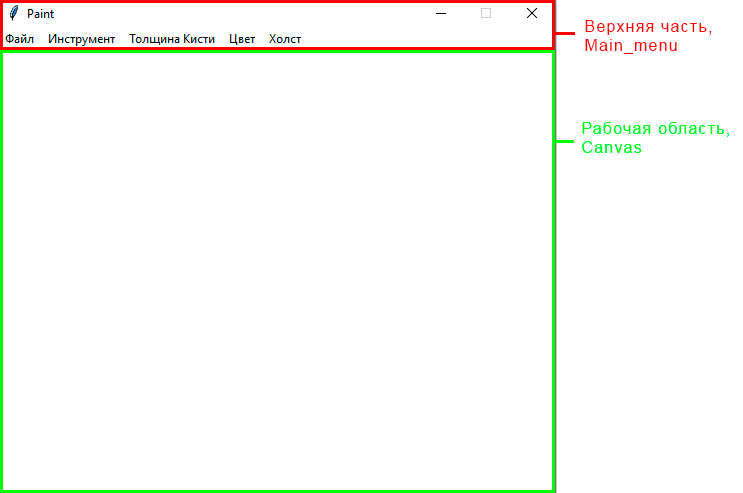
\includegraphics[width=1\linewidth]{shablon}
\caption{Композиция шаблона приложения}
\label{shablon:image}
\end{figure}
%\vspace{-\figureaboveskip} % двойной отступ не нужен (можно использовать, если раздел заканчивается картинкой)

\subsection{Моделирование вариантов использования}

Для разрабатываемого приложения была реализована модель, которая обеспечивает наглядное представление вариантов использования приложения.

Она помогает в физической разработке и детальном анализе взаимосвязей объектов. При построении диаграммы вариантов использования применяется унифицированный язык визуального моделирования UML.

Диаграмма вариантов описывает функциональное назначение разрабатываемой системы. То есть это то, что система будет непосредственно делать в процессе своего функционирования. Она является исходным концептуальным представлением системы в процессе ее проектирования и разработки. Проектируемая система представляется в виде ряда прецедентов, предоставляемых системой актерам или сущностям, которые взаимодействуют с системой. Актером или действующим лицом является сущность, взаимодействующая с системой извне (например, человек, техническое устройство). Прецедент служит для описания набора действий, которые система предоставляет актеру.

На основании анализа предметной области в программе должны быть реализованы следующие прецеденты:
\subsubsection{Первый запуск}

При первом запуске программы пользователь должен выбрать ширину и высоту будущего изображения в начальном окне. Если введенные данные корректны, то пользователь получает доступ к основному окну.

\subsubsection{Сохранение}

При нажатии пользователем кнопки «Сохранить», открывается диалоговое окно, в котором пользователь должен выбрать имя и путь к изображению.

\subsubsection{Открытие}

При нажатии пользователем кнопки «Открыть», открывается диалоговое окно, в котором пользователь должен выбрать уже существующее изображение для редактирования.

\subsubsection{Рисование}

При нажатии в рабочую зону левой кнопкой мыши, появляется точка определенного радиуса. Если пользователь будет удерживать левую кнопку мыши, то точки, появляющиеся в рабочей зоне, начнут соединяться, образуя линии.

\subsubsection{Смена размера}

При выборе любого пункта в разделе «Толщина кисти», пользователь изменяет радиус создаваемой точки из прецедента «Рисование».

\subsubsection{Смена цвета}

При выборе любого пункта в разделе «Цвет», пользователь изменяет цвет создаваемой точки из прецедента «Рисование».

\subsubsection{Цвет холста}

При выборе пункта «Цвет холста», пользователь изменяет цвет всей рабочей зоны на выбранный.

\subsubsection{Очистка холста}

При выборе пункта «Очистка холста», пользователь изменяет цвет всей рабочей зоны на белый.

\subsection{Требования к оформлению документации}

Разработка программной документации и программного изделия должна производиться согласно ГОСТ 19.102-77 и ГОСТ 34.601-90. Единая система программной документации.

\section{Технический проект}
\subsection{Общая характеристика организации решения задачи}

Необходимо спроектировать и разработать приложение, с помощью которого можно редактировать различные изображения.

Графический редактор представляет собой программное средство, разработанное для создания, редактирования и обработки графических изображений. Он предоставляет пользователю набор инструментов и функций для работы с различными видами графики, включая рисунки, фотографии, иллюстрации и другие визуальные материалы.

\subsection{Обоснование выбора технологии проектирования}

На сегодняшний день информационный рынок, поставляющий программные решения в выбранной сфере, предлагает множество продуктов, позволяющих достигнуть поставленной цели – разработки графического редактора.

\subsubsection{Описание используемых технологий и языков программирования}

В процессе разработки графического редактора используются программные средства и языки программирования. Каждое программное средство применяется для круга задач, при решении которых оно необходимо.

\subsubsection{Язык программирования Python}

Python — высокоуровневый язык программирования общего назначения с динамической строгой типизацией и автоматическим управлением памятью, ориентированный на повышение производительности разработчика, читаемости кода и его качества, а также на обеспечение переносимости написанных на нём программ.

\paragraph{Достоинства языка Python}

Простота и читаемость: Python известен своей простотой синтаксиса, что делает его легким для изучения и понимания. Читаемый код способствует совместной работе и обслуживанию.

Множество библиотек и фреймворков: Python обладает обширным экосистемой библиотек и фреймворков, что упрощает разработку приложений в различных областях, таких как веб-разработка, научные вычисления, машинное обучение и другие.

Портативность: Python поддерживает множество платформ, что позволяет запускать программы на различных операционных системах без изменений в коде.

\paragraph{Недостатки языка Python}

Производительность в некоторых случаях: В сравнении с некоторыми компилируемыми языками, Python может быть менее производительным, особенно в задачах, требующих высокой вычислительной мощности.

Глобальная блокировка интерпретатора (GIL): GIL ограничивает одновременное выполнение нескольких потоков в Python, что может быть проблемой в многопоточных приложениях.

Объем занимаемой памяти: Python может потреблять больше памяти по сравнению с некоторыми другими языками.

\subsection{Диаграмма компонентов и схема обмена данными между файлами компонента}

Диаграмма компонентов описывает особенности физического представления разрабатываемого приложения. Она позволяет определить архитектуру системы, установив зависимости между программными компонентами, в роли которых может выступать как исходный, так и исполняемый код. Основными графическими элементами диаграммы компонентов являются компоненты, интерфейсы, а также зависимости между ними. На рисунке \ref{compo:image} изображена диаграмма компонентов для проектируемого приложения. Она включает в себя начальное и основное окно, в котором находятся компоненты «Холст» и «Инструмент». Инструментом может быть: кисть, карандаш или ластик.

\begin{figure}[ht]
\center{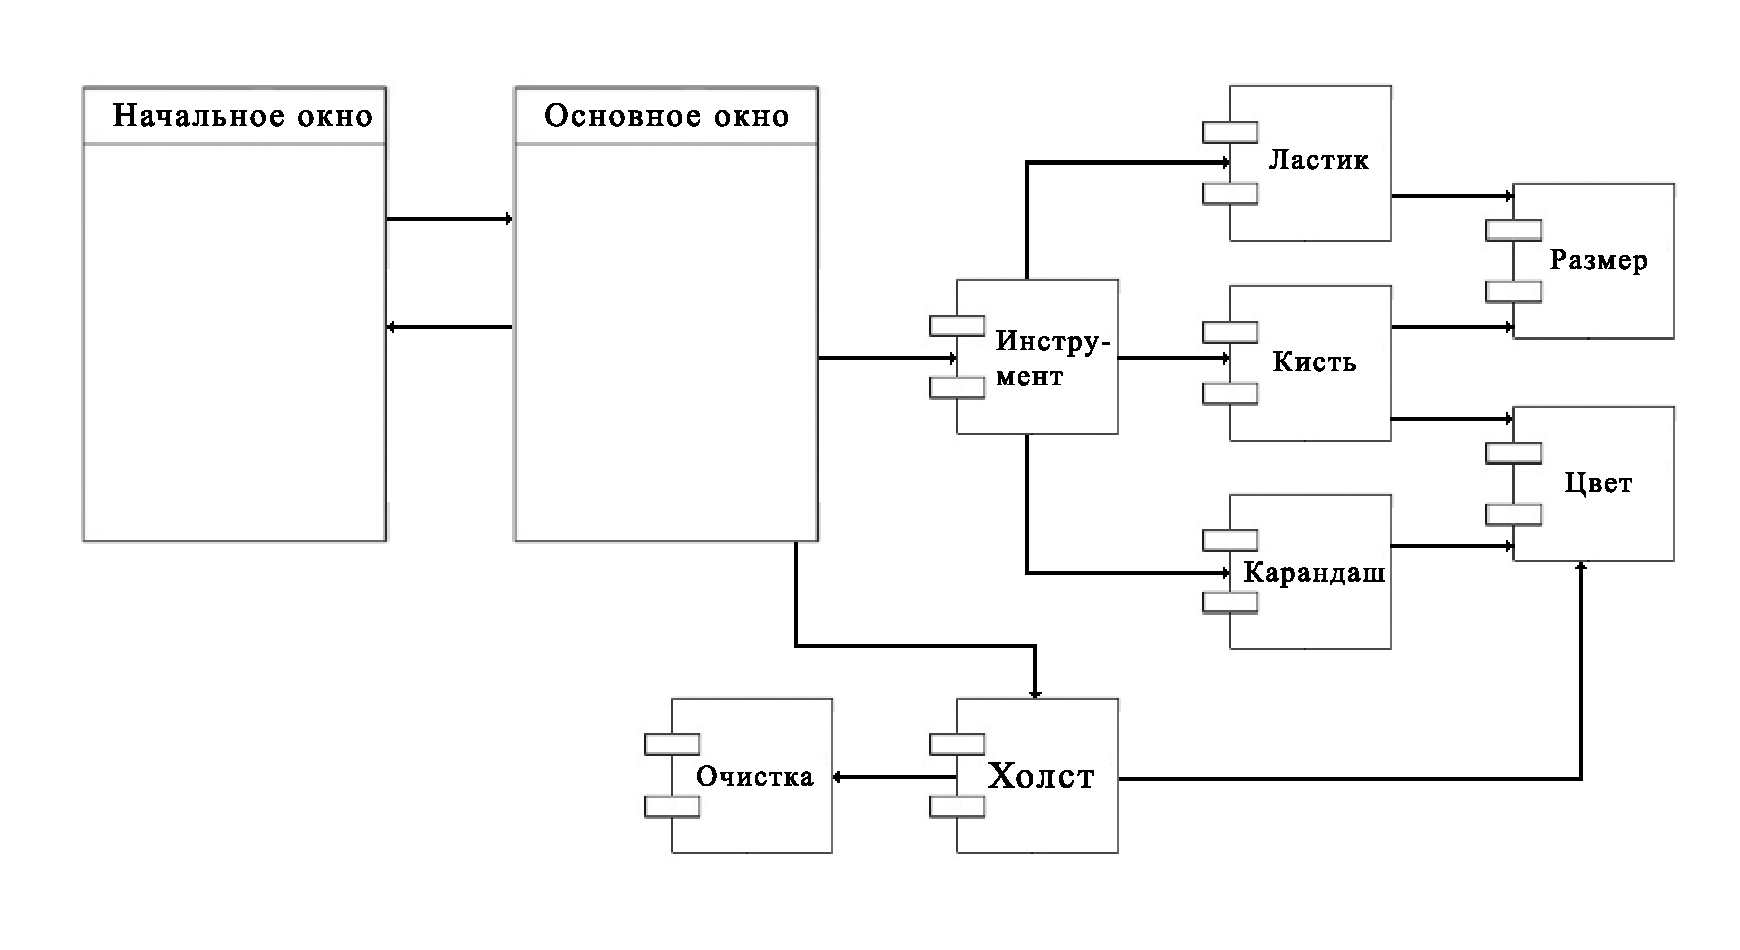
\includegraphics[width=1\linewidth]{compo}}
\caption{Диаграмма компонентов}
\label{compo:image}
\end{figure}

Любой компонент должен быть вызван в сценарии редактора. Редактор передает данные компоненту в момент вызова последнего.

На рисунке \ref{cp2:image} представлена схема обмена данными между сценариями редактора при взаимодействии компонентов.

\begin{figure}[ht]
\center{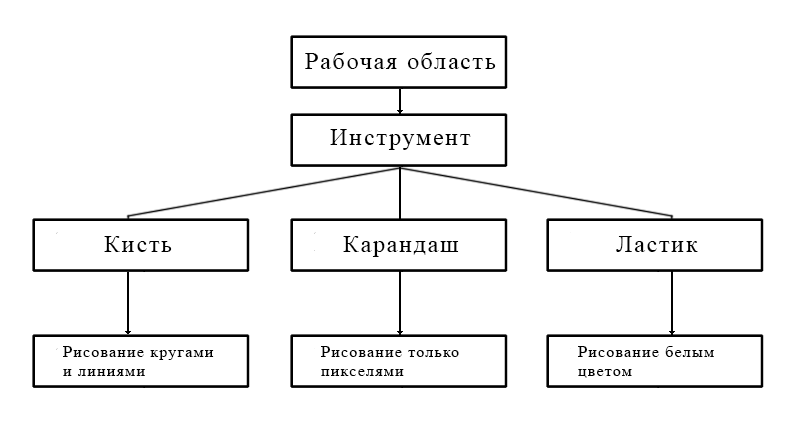
\includegraphics[width=1\linewidth]{cp2}}
\caption{Диаграмма компонентов}
\label{cp2:image}
\end{figure}

При взаимодействии с компонентом в сценарии редактора происходит распознавание взаимодействующих объектов.
Если пользователь выберет объект «Кисть», то он перейдет в обычный режим рисования. Нажатием левой кнопки мыши, он будет создавать круги, которые соединяются между собой линиями. Если пользователь выберет объект «Карандаш», то он перейдет в режим рисования пикселями. Взаимодействие с рабочей зоной будет создавать на ней единичные пиксели. Если пользователь выберет объект «Ластик», то он сменит цвет своей кисти на белый.

Работа компонента заканчивается в момент завершения работы сценария редактора.

\subsection{Содержание информационных блоков. Основные сущности}

Проанализировав требования, можно выделить одну основную сущность:
\begin{itemize}
\item "<Кисточка">;
\end{itemize}

В состав сущности "<Кисточка"> можно включить атрибуты, представленные в таблице \ref{news:table}.

\begin{xltabular}{\textwidth}{|l|l|p{1.7cm}|X|}
	\caption{Атрибуты сущности "<Кисточка">\label{news:table}}\\ \hline
	\centrow Поле & \centrow Тип & \centrow Обяза\-тельное & \centrow Описание \\ \hline
	\thead{1} & \thead{2} & \centrow 3 & \centrow 4 \\ \hline
	\endfirsthead
	\continuecaption{Продолжение таблицы \ref{news:table}}
	\thead{1} & \thead{2} & \centrow 3 & \centrow 4 \\ \hline
	\finishhead
	color & str & true & Цвет кисти \\ \hline 
	brush\_size & int & true & Размер кисти \\ \hline 
	lcolor & str & false & Предыдущий цвет кисти \\ \hline 
	pixel\_flag & bool & true & Тип кисти \\ \hline 
	lx & list & true & Список x координат кисти \\ \hline 
	ly & list & true & Список y координат кисти
\end{xltabular}



\ifПрактика{}\else{
   \section{Рабочий проект}
\subsection{Классы, используемые при разработке приложения}

Можно выделить следующий список классов и их методов, использованных при разработке приложения (таблица \ref{class:table}). 

\renewcommand{\arraystretch}{0.8} % уменьшение расстояний до сетки таблицы
\begin{xltabular}{\textwidth}{|X|p{2.5cm}|>{\setlength{\baselineskip}{0.7\baselineskip}}p{4.85cm}|>{\setlength{\baselineskip}{0.7\baselineskip}}p{4.85cm}|}
	\caption{Описание классов, используемых в приложении\label{class:table}}\\
	\hline \centrow \setlength{\baselineskip}{0.7\baselineskip} Название класса & \centrow \setlength{\baselineskip}{0.7\baselineskip} Модуль, к которому относится класс & \centrow Описание класса & \centrow Методы \\
	\hline \centrow 1 & \centrow 2 & \centrow 3 & \centrow 4\\ \hline
	\endfirsthead
	\caption*{Продолжение таблицы \ref{class:table}}\\
	\hline \centrow 1 & \centrow 2 & \centrow 3 & \centrow 4\\ \hline
	\finishhead
	MainWindow & Главный модуль & MainWindow – главный класс приложения. Содержит основные функции для создания и взаимодействия с рабочей областью. & create\_root(self, cwidth, cheight, fo, sImg)
	Cоздает основное окно, которое состоит из меню и канваса
	paint(event, self)
	Отрисовывает круги в месте клика мышки
	brelease(event, self)
	Очищает созданные списки
	cr\_line(event, self)
	Соединяет два отрисованных круга линией\\
	\hline 
	FirstWindow & Доп. модуль & FirstWindow – класс, создающий начальное окно с вводом параметров изображения. & firstroot(self)
	Создает начальное окно 
	check\_var(self)
	Проверяет значение вводимых переменных
	create\_newImg(self)
	Уничтожает начальное окно и вызывает функцию для создания основного\\
	\hline
	Inter & Доп. модуль & Inter – класс, отвечающий за сохранение и открытие других изображений. & save\_img(self)
	Сохраняет изображение
	open\_img(self)
	Открывает изображение
	createImg(self)
	Вызывает начальное окно
	w\_and\_h(self, fname)
	Узнает размеры, открываемого изображения\\
	\hline
	Brush & Доп. модуль & Brush – класс, отвечающий за параметры кисти. & eraser(self)
	Меняет цвет кисти на белый
	size\_change(self, new\_size)
	Меняет радиус кисти на выбранный
	color\_change(self)
	Меняет цвет кисти на выбранный
	clear\_canvas(self, f)
	Полностью очищает canvas
	pour(self, f)
	Полностью очищает canvas, устанавливает фон с таким же цветом, как и у кисти
	brush(self)
	Выбирает режим обычного рисования
	pixel\_brush(self)
	Выбирает режим пиксельного рисования
	eraser(self)
	Меняет цвет кисти на белый \\
	\hline
\end{xltabular}
\renewcommand{\arraystretch}{1.0} % восстановление сетки

\subsection{Системное тестирование разработанного приложения}

На рисунке \ref{osn:image} представлено основное окно графического редактора.
\newpage % при необходимости можно переносить рисунок на новую страницу
\begin{figure}[H] % H - рисунок обязательно здесь, или переносится, оставляя пустоту
\center{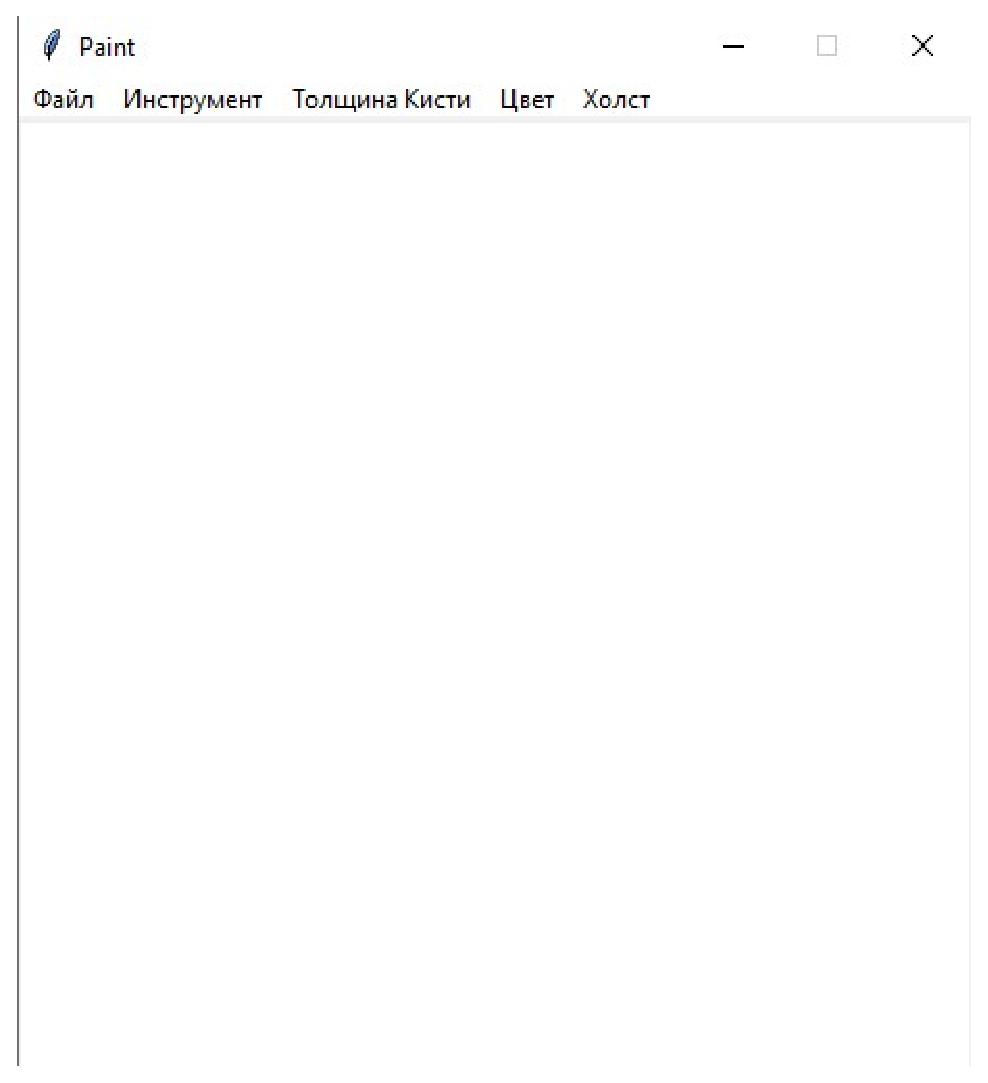
\includegraphics[width=1\linewidth]{osn}}
\caption{Основное окно}
\label{osn:image}
\end{figure}

На рисунке \ref{vvod:image} представлено начальное окно с выбором параметров будущего изображения.

\begin{figure}[H]
\center{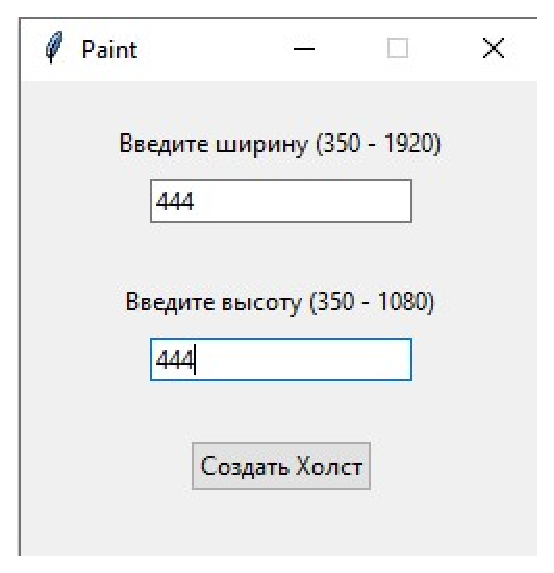
\includegraphics[width=1\linewidth]{vvod}}
\caption{Начальное окно}
\label{vvod:image}
\end{figure}

На рисунке \ref{sve:image} представлено сохранение файла через диалоговое окно.

\begin{figure}[H]
\center{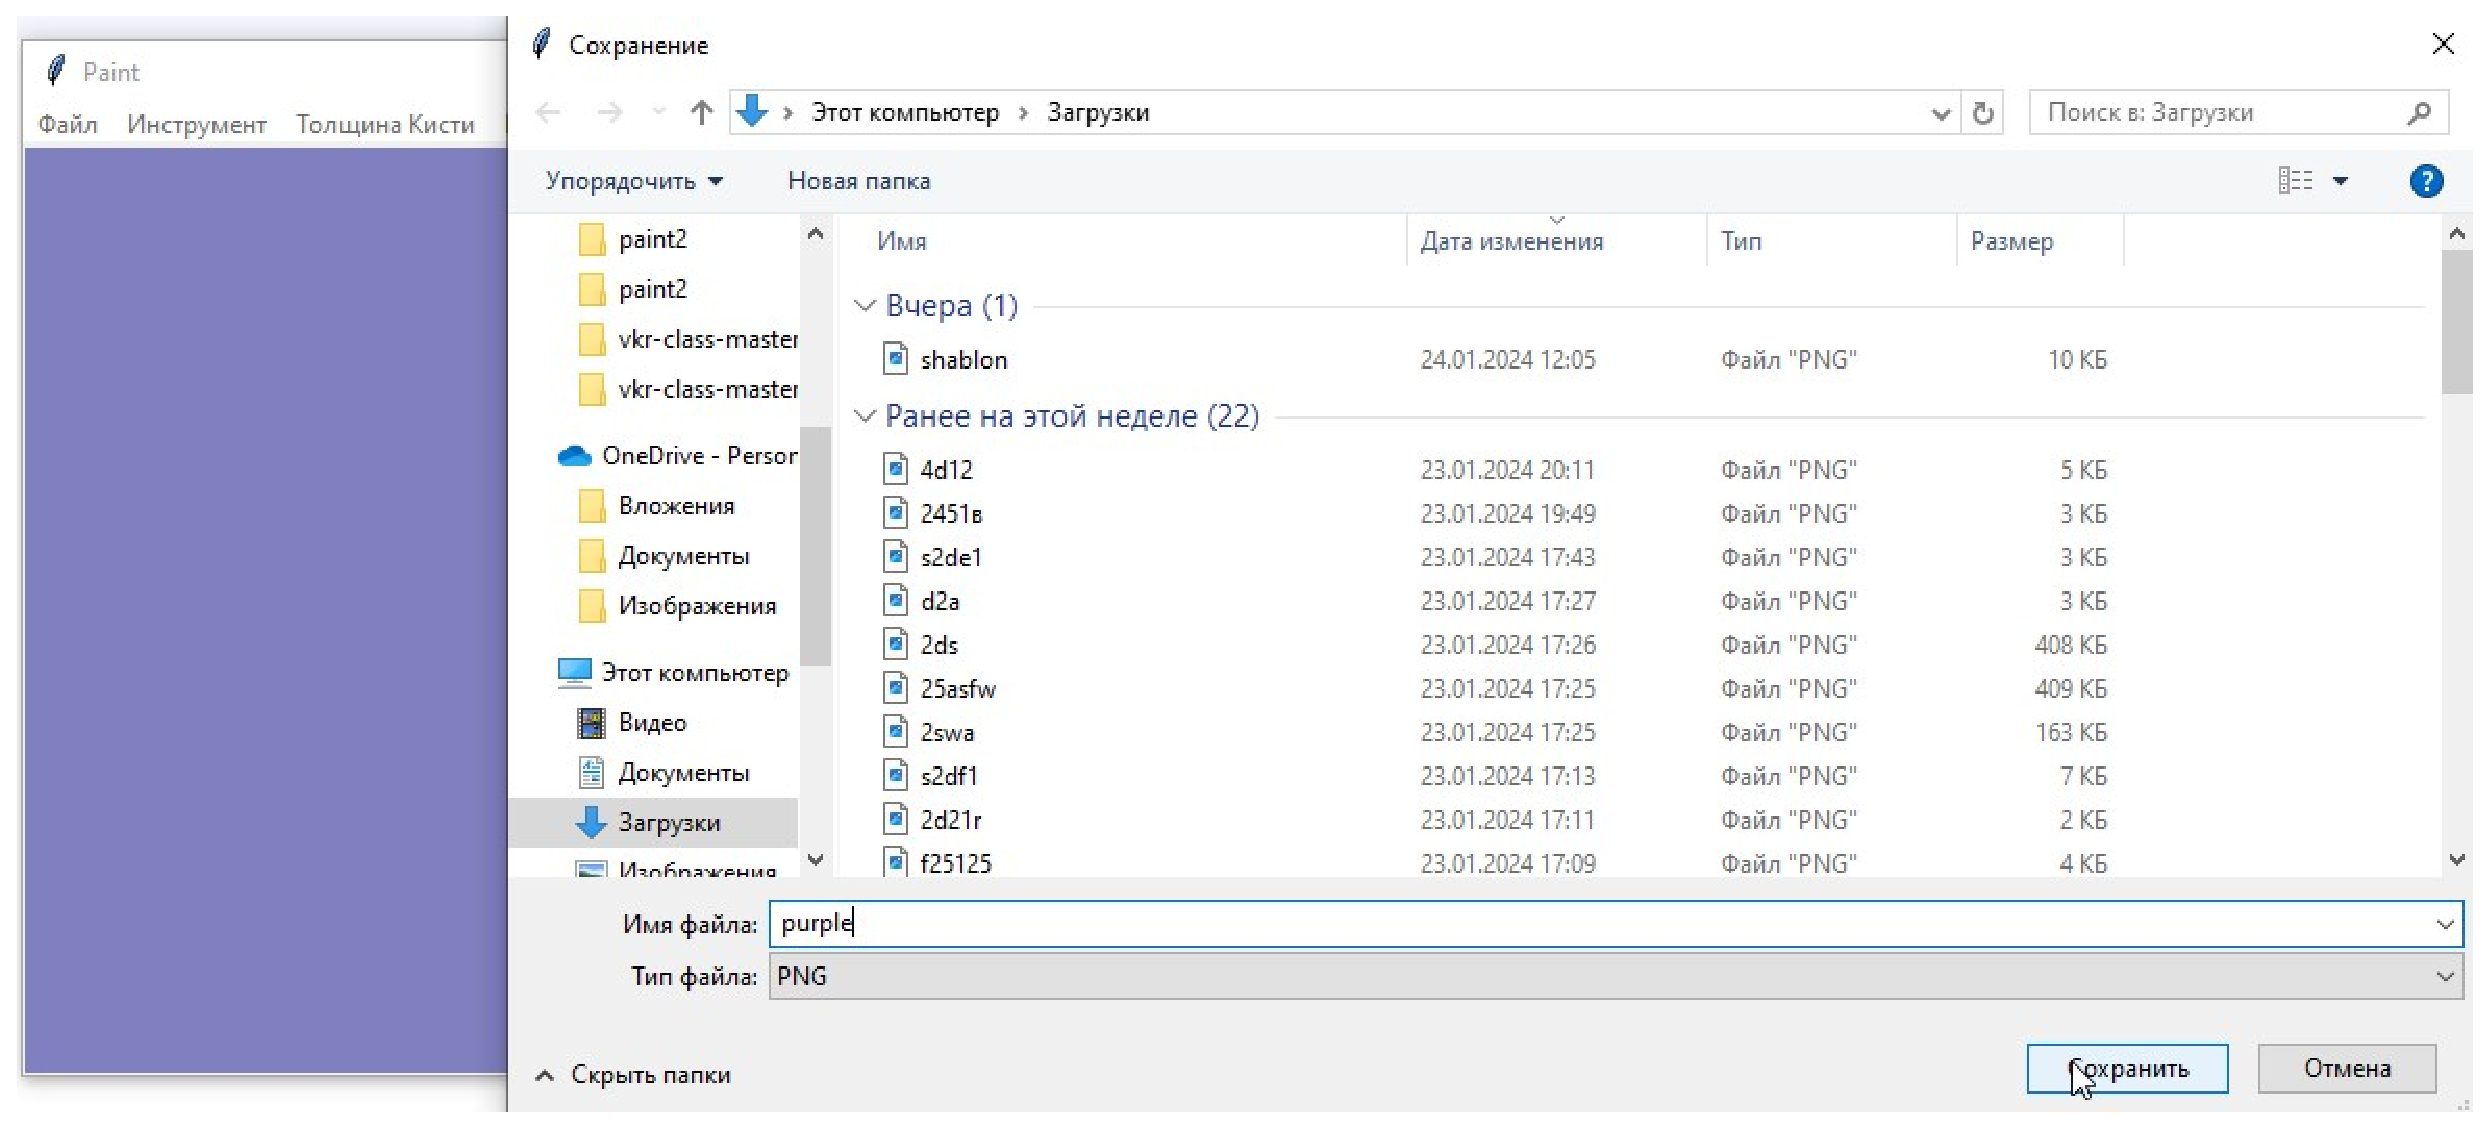
\includegraphics[width=1\linewidth]{sve}}
\caption{Сохранение файла}
\label{sve:image}
\end{figure}

На рисунке \ref{ope:image} представлено открытие файла через диалоговое окно.

\begin{figure}[H]
	\center{\includegraphics[width=1\linewidth]{ope}}
	\caption{Открытие файла}
	\label{ope:image}
\end{figure}

На рисунке \ref{size:image} представлено изменение размера кисти пользователем.

\begin{figure}[H]
	\center{
\includegraphics[width=1\linewidth]{size}}
	\caption{Изменение размера кисти}
	\label{size:image}
\end{figure}

На рисунке \ref{clr:image} представлено изменение цвета кисти пользователем.

\begin{figure}[H]
	\center{
\includegraphics[width=1\linewidth]{clr}}
	\caption{Изменение цвета кисти}
	\label{clr:image}
\end{figure}

На рисунке \ref{hlst:image} представлена заливка всей рабочей зоны определенным цветом.

\begin{figure}[H]
	\center{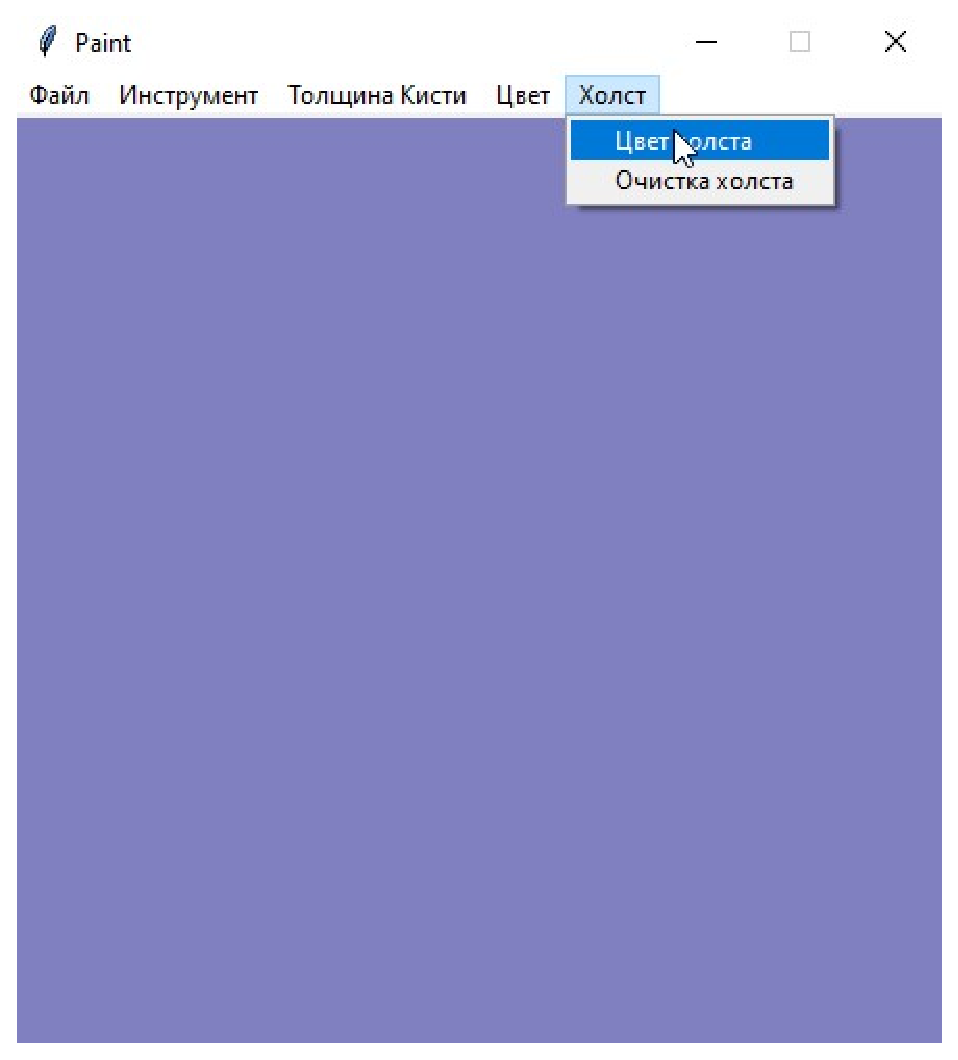
\includegraphics[width=1\linewidth]{hlst}}
	\caption{Заливка холста}
	\label{hlst:image}
\end{figure}

   \section*{ЗАКЛЮЧЕНИЕ}
\addcontentsline{toc}{section}{ЗАКЛЮЧЕНИЕ}

Основной целью работы было создание интуитивно понятного графического редактора, способного удовлетворять потребности пользователей в обработке изображений. В ходе реализации проекта были определены ключевые компоненты и их взаимодействие. Важным этапом работы было проектирование удобного пользовательского интерфейса, который бы обеспечивал взаимодействие пользователя с редактором.

Реализация графического редактора включала в себя создание инструментов для рисования, редактирования и обработки изображений. Процесс разработки включал в себя тестирование функционала, что позволило выявить и устранить потенциальные ошибки.

Основные результаты работы:

\begin{enumerate}
\item Проведен анализ предметной области.
\item Разработана модель данных системы. Определены требования к системе.
\item Разработана архитектура приложения. Разработан пользовательский интерфейс приложения.
\item Приложение реализовано и протестировано. Проведено системное тестирование.
\end{enumerate}

Все требования, объявленные в техническом задании, были полностью реализованы, все задачи, поставленные в начале разработки проекта, были также решены.

}\fi
\addcontentsline{toc}{section}{СПИСОК ИСПОЛЬЗОВАННЫХ ИСТОЧНИКОВ}

\begin{thebibliography}{9}

    \bibitem{python_pocket_guide_online}
    Джиджак, Э. Python. Эффективное программирование. – ДМК Пресс, 2020. – 720 с. – ISBN 978-5-97060-824-0. – Текст~: прямой.
    \bibitem{python_mastering}
    Ван Розум, Г. Python. К вершинам мастерства / Г. Ван Розум. – БХВ-Петербург, 2019. – 672 с. – ISBN 978-5-4461-1360-3. – Текст~: прямой.
    \bibitem{python_data_science_book}
    Бизли, Д. Python. Наука о данных / Д. Бизли. – ДМК Пресс, 2019. – 384 с. – ISBN 978-5-97060-603-1. – Текст~: прямой.
    \bibitem{python_complex_tasks}
    Доусон, М. Python для сложных задач. Основы программирования / М. Доусон. – ДМК Пресс, 2020. – 512 с. – ISBN 978-5-907114-33-4. – Текст~: прямой.
    \bibitem{fluent_python_course}
    ВандерПлас, Дж. Fluent Python. Курс современного программиста / Дж. ВандерПлас. – ДМК Пресс, 2021. – 656 с. – ISBN 978-5-907114-94-5. – Текст~: прямой.
    \bibitem{python_comprehensive_guide}
    Мэтсес, Э. Python. Подробное руководство / Э. Мэтсес. – ДМК Пресс, 2016. – 528 с. – ISBN 978-5-94074-943-7. – Текст~: прямой.
    \bibitem{python_useful}
    Любанович, Б. Python. Самое необходимое / Б. Любанович. – Питер, 2018. – 352 с. – ISBN 978-5-496-02659-2. – Текст~: прямой.
    \bibitem{python_data_science}
    Саммерфильд, М. Программирование на Python в науках о данных / М. Саммерфильд. – ДМК Пресс, 2021. – 576 с. – ISBN 978-5-97060-987-2. – Текст~: прямой.
    \bibitem{python_express_course}
    Бейдер, Д. Python. Экспресс-курс / Д. Бейдер. – Питер, 2020. – 256 с. – ISBN 978-5-4461-1280-4. – Текст~: прямой.
    \bibitem{python_data_analysis}
    Маккини, У. Python и анализ данных / У. Маккини. – ДМК Пресс, 2017. – 536 с. – ISBN 978-5-97060-348-1. – Текст~: прямой.
    
\end{thebibliography}

\ifВКР{\appendix{Представление графического материала}

Графический материал, выполненный на отдельных листах,
изображен на рисунках А.1--А.\arabic{числоПлакатов}.
\setcounter{числоПлакатов}{0}

\renewcommand{\thefigure}{А.\arabic{figure}} % шаблон номера для плакатов

\begin{landscape}

\begin{плакат}
    
\includegraphics[width=0.82\linewidth]{плакат1.png}
    \заголовок{Сведения о ВКРБ}
    \label{pl1:image}      
\end{плакат}

\begin{плакат}
    
\includegraphics[width=0.82\linewidth]{плакат2.png}
    \заголовок{Цель и задачи разработки}
    \label{pl2:image}      
\end{плакат}

\begin{плакат}
    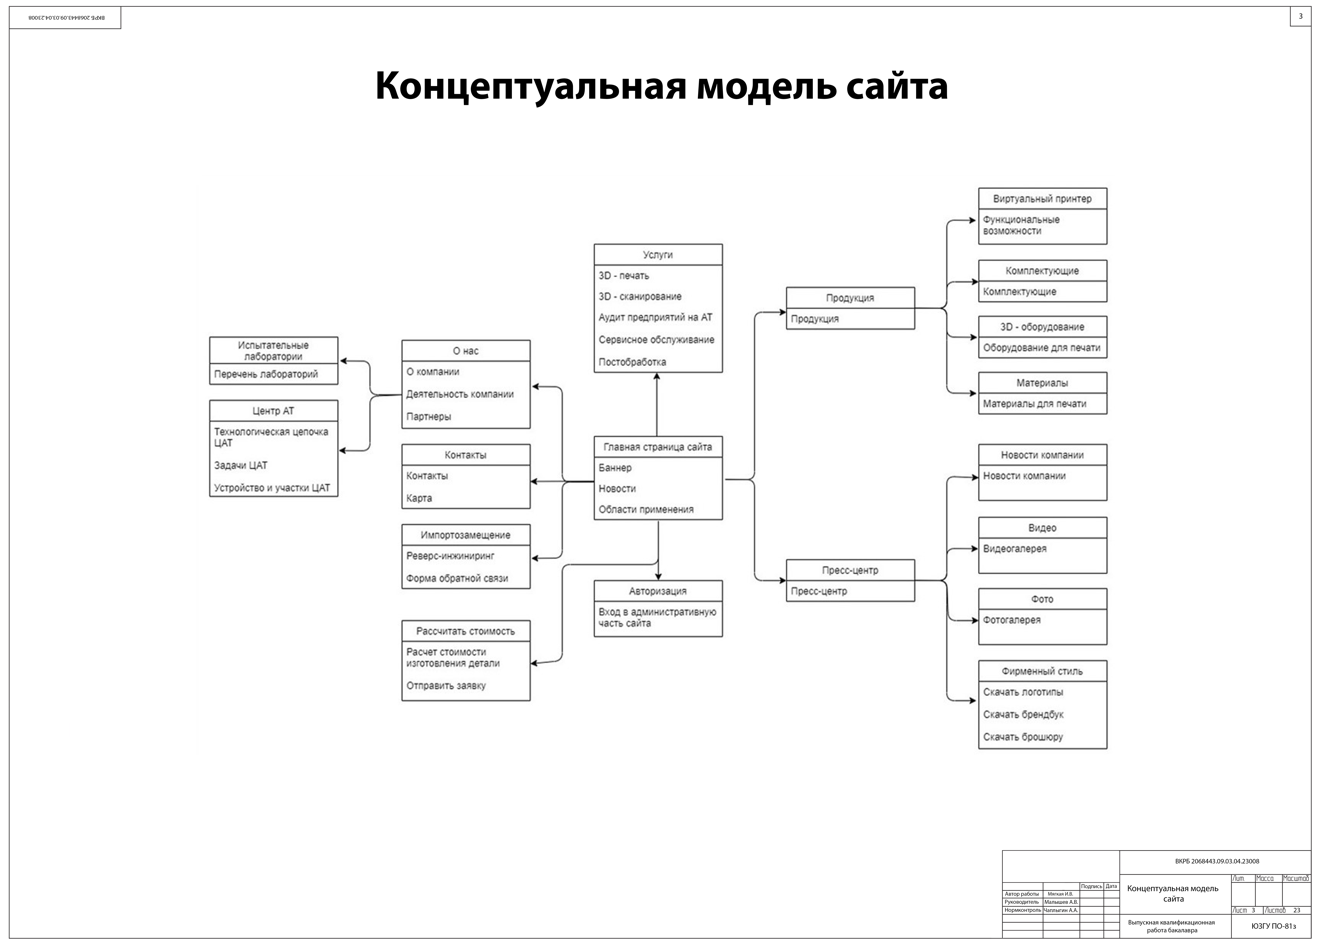
\includegraphics[width=0.82\linewidth]{плакат3.png}
    \заголовок{Концептуальная модель сайта}
    \label{pl3:image}      
\end{плакат}

\begin{плакат}
    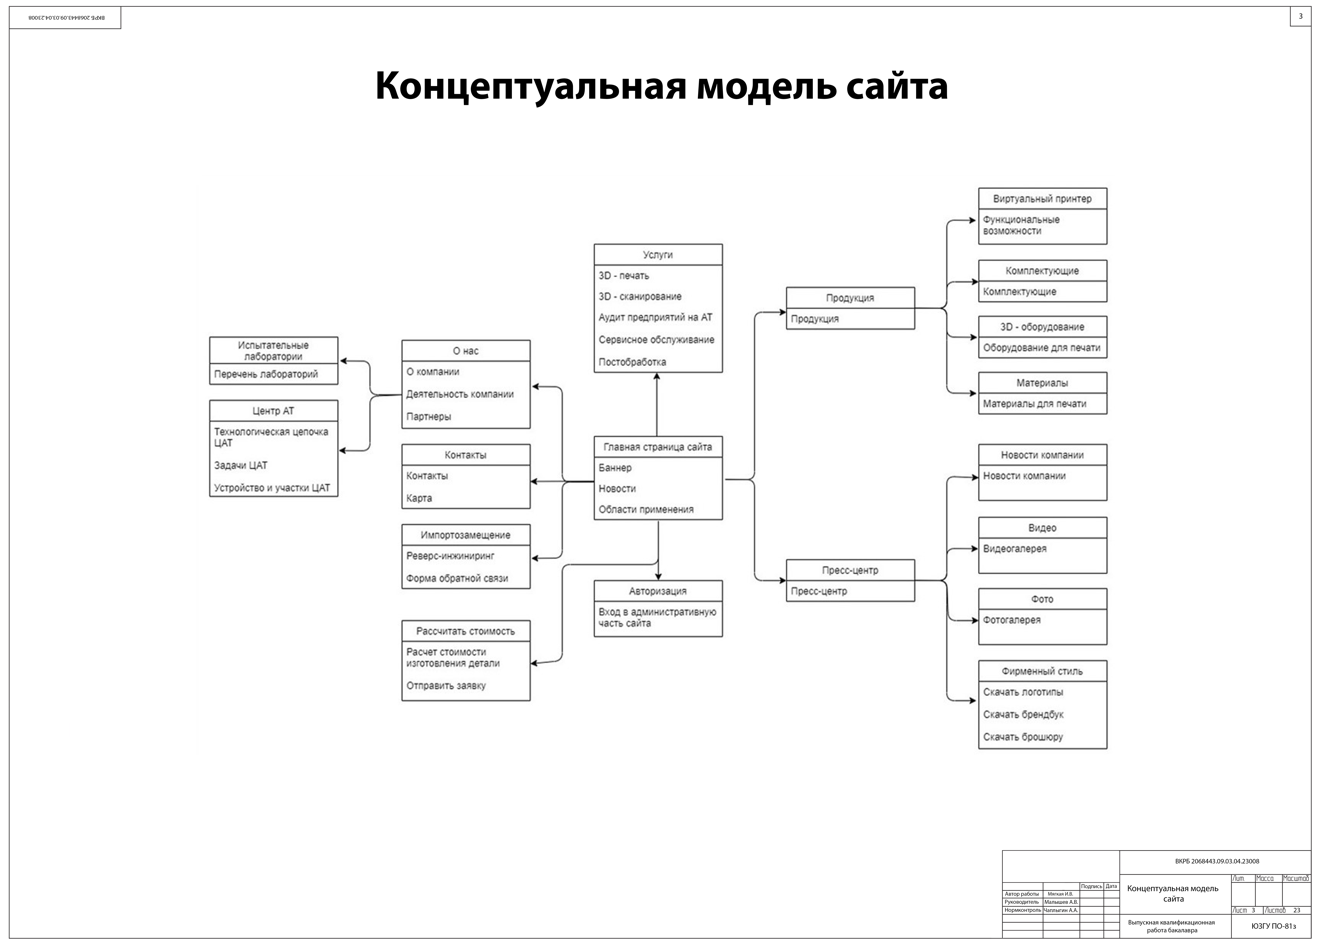
\includegraphics[width=0.82\linewidth]{плакат3.png}
    \заголовок{Еще плакат}
    \label{pl4:image}      
\end{плакат}

\end{landscape}
}\fi
\ifПрактика{}\else{\appendix{Фрагменты исходного кода программы}

main.py
\lstinputlisting[language=Python, frame=none]{main.py}

mwindow.py
\lstinputlisting[language=Python, frame=none]{mwindow.py}

fwindow.py
\lstinputlisting[language=Python, frame=none]{fwindow.py}

brushes.py
\lstinputlisting[language=Python, frame=none]{brushes.py}

interaction.py
\lstinputlisting[language=Python, frame=none]{interaction.py}


\ifВКР{
\newpage
\addcontentsline{toc}{section}{На отдельных листах (CD-RW в прикрепленном конверте)}
\begin{center}
\textbf{Место для диска}
\end{center}
}\fi
}\fi
\end{document}
